\documentclass[letterpaper]{article} % DO NOT CHANGE THIS
\usepackage[submission]{aaai2027} % DO NOT CHANGE THIS
\usepackage[hyphens]{url}
\usepackage{graphicx}
\urlstyle{rm}
\def\UrlFont{\rm}
\usepackage{natbib}
\usepackage{caption}
\usepackage{booktabs}
\usepackage{amsmath}
\usepackage{xspace}
\frenchspacing
\setcounter{secnumdepth}{2}
\newcommand{\carp}{\textsc{CARP}\xspace}
\newcommand{\asl}{\textsc{ASL}\xspace}

\pdfinfo{
/TemplateVersion (2027.1)
}

\title{Supplementary Material:\\Unidentified, yet Linkable?}
\author{Anonymous Submission}
\affiliations{}

\begin{document}
\maketitle

\section{Purpose and Scope}

This supplement separates implementation details from the main paper's conceptual description.
It records the complete reference-attack contract, parameter choices, calibration boundaries,
dataset limitations, learned-representation comparisons, and the observation-equivalence analysis.
The code and machine-readable tables are included in the anonymous artifact.

\section{Reference-Attack Contract}

\carp is an interpretable reference attack composed from established blocking, similarity,
union--find, and connected-component primitives. It is not presented as a new graph-learning or
entity-resolution primitive. Given identifier-stripped provider-visible requests, a pair budget,
and a typed-handle vocabulary, it:
\begin{enumerate}
  \item extracts bounded structural, continuity, timing, and tool features;
  \item groups requests into optional cache-like blocks;
  \item creates local candidates using bounded inverted indexes;
  \item applies deterministic session and typed-entity edge rules;
  \item builds separate session, user/customer, project/process, and tenant/owner components;
  \item rejects shared-resource and alias-bridging ambiguity;
  \item propagates unambiguous typed handles across blocks; and
  \item optionally assigns later requests to an early-traffic watchlist.
\end{enumerate}

\subsection{Shared Parameters}

\begin{table*}[t]
\centering
\small
\begin{tabular}{@{}llll@{}}
\toprule
Stage & Parameter & Value & Purpose \\
\midrule
Rare session index & maximum bucket & 20 & exclude common trace values \\
User/customer index & maximum bucket & 80 & bound exact customer anchors \\
Project/owner index & maximum bucket & 400 & bound repository/business anchors \\
Semantic candidates & maximum bucket & 20 & local signature blocking \\
Shingle candidates & maximum bucket & 35 & cumulative-context blocking \\
Refinement candidates & maximum bucket & 20 & local multi-signal comparison \\
All local passes & pair budget/request & 400 & cap candidate materialization \\
Semantic edge & signatures/Jaccard/IDs/gap & $2/.32/3/90$ min & default semantic rule \\
Context edge & containment/Jaccard/IDs/repo & $.78/.20/2/1$ & context-growth rule \\
Context edge & maximum gap & 180 min & context-growth rule \\
Refinement A & Jaccard/IDs/gap & $.22/2/180$ min & session rule \\
Refinement B & Jaccard/semantic/IDs/gap & $.24/2/3/90$ min & session rule \\
\bottomrule
\end{tabular}
\caption{Shared implementation parameters. These values are engineering settings, not universal
constants or claims about an optimal linkage rule.}
\end{table*}

The main Open-SWE run disables the optional semantic-signature pass because its development-slice
ablation leaves the result unchanged. Large streamed overlay runs cap each request at 24K characters,
1,200 shingles, and 1,500 words. The standard extraction caps are 80K characters, 8K shingles, and
5K words. Candidate and threshold sensitivity are reported separately rather than treating the
defaults as theoretically privileged.

\subsection{Protocol-Specific Calibration}

\begin{table*}[t]
\centering
\small
\begin{tabular}{@{}p{0.22\textwidth}p{0.34\textwidth}p{0.36\textwidth}@{}}
\toprule
Protocol & Calibration/fixed setting & Evaluation boundary \\
\midrule
Open-SWE main & local rules checked on 100 development workflows; semantic pass disabled & 900 workflows, turns 3/6/9/12 \\
Historical tau default & shared CARP rules transferred without retuning & 160 held-out workflows \\
Historical tau high precision & maximum calibration F1 subject to precision $\geq .8$ & 40 calibration, 160 held-out workflows \\
Controlled tau overlay & deterministic typed schema and ambiguity rule fixed on early traffic & first 2,500 requests for cold start; later traffic scored separately \\
Non-code content stage & identifier-masked initial intent, MiniLM top-24, cosine .98 & 40 calibration, 160 held-out workflows \\
Strict Open-SWE project stage & 40K TF--IDF vocabulary, MiniLM weight .50, sparse floor .20, threshold .44, top-24 & 160 calibration projects, 479 unseen projects \\
Cross-scaffold transfer & source-selected representation weight, threshold quantile, and ambiguity margin & target labels never used; both directions evaluated \\
HNSW & cosine, $M=16$, efConstruction 200, efSearch 16/64/200, top-24 & 1,736 held-out tau requests \\
\bottomrule
\end{tabular}
\caption{Calibration and evaluation boundaries.}
\end{table*}

\section{Agent-State Linkage Contract}

\asl is an experimental selective extension kept separate from the frozen \carp implementation.
For each request it retains fixed-cap hashes and counts for message-event replay, initial task,
recent context, tool observations, action classes, errors, resource fingerprints and roots, and
level-typed handles. It deliberately omits raw message text from the retained hot-path state. The
streaming index caps each posting list at 64, candidates per request at 96, and active history at 90
minutes. Overfull keys become suppressed heavy hitters rather than unbounded buckets.

Candidate scoring separates support from conflict. Support may come from directed replay
containment, initial-task agreement, typed-handle overlap, tool/resource continuity, shared resource
roots, and ordered progression. Hard conflicts include time reversal, incompatible strong user or
tenant handles, and competing initial roots. Acceptance requires score 4.2, at least three evidence
families, no hard conflict, and best-versus-runner-up margin .35. Resource-root edges without full
replay additionally require ordered tool/resource progression and at least two resource matches.
The 90-minute gap is a workflow boundary only; persistent typed handles may still connect completed
workflow summaries at the corresponding user, project, or tenant level.

\begin{table*}[t]
\centering
\small
\begin{tabular}{@{}llrrrrrr@{}}
\toprule
Dataset & Method & Prec. & Rec. & F1 & Coverage & Abstain & Contam. req. \\
\midrule
Open-SWE delta (400) & CARP & .474 & .060 & .107 & --- & --- & --- \\
 & Generic hashed text & 1.000 & .113 & .204 & --- & .848 & 0 \\
 & ASL & 1.000 & .245 & .394 & .390 & .703 & 0 \\
Historical tau (2,175) & CARP & .975 & .055 & .104 & --- & --- & --- \\
 & Generic hashed text & .938 & .010 & .019 & --- & .955 & 11 \\
 & ASL & 1.000 & .090 & .164 & .374 & .646 & 0 \\
\bottomrule
\end{tabular}
\caption{Agent-state feasibility slices. Coverage is the fraction of recoverable predecessor edges
accepted correctly; contamination counts requests in mixed predicted components. These diagnostic
slices are separate from the paper's primary held-out matrix.}
\end{table*}

Evidence ablations expose different Agent traffic forms. On Open-SWE delta windows, replay-only,
tool/resource-only, and typed-handle-only F1 are .000/.363/.010: continuity lies mainly in tool and
workspace state crossing adjacent windows. On cumulative tau requests the corresponding values are
.035/.000/.066, while their combination reaches .164. Removing conflicts leaves the strict
operating-point results unchanged on both slices, so conflict rejection is supported by adversarial
fixtures rather than claimed as an empirical gain here. The generic control uses a 32,768-dimensional
hashing vectorizer and cosine nearest neighbor in the same active window. It requires 20.0/61.7
comparisons per request on Open-SWE/tau, versus 5.1/24.0 for \asl's typed indexes.

\begin{table}[t]
\centering
\small
\begin{tabular}{@{}rrrrrr@{}}
\toprule
Requests & Seconds & Req./s & Active states & Postings & RSS MiB \\
\midrule
10K & 3.68 & 2,714 & 1,801 & 17,716 & 41 \\
100K & 38.99 & 2,565 & 1,801 & 17,716 & 118 \\
500K & 188.82 & 2,648 & 1,801 & 17,716 & 435 \\
\bottomrule
\end{tabular}
\caption{Controlled \asl computation scale. Active retrieval is bounded; required output labels
and union--find state grow linearly.}
\end{table}

\section{Fidelity-Certified Trace Reconstruction}

Dataset evidence is labeled by fidelity rather than collectively called real traffic: F3 is an
exact API payload, F2 a framework-faithful reconstruction, F1 a trajectory-prefix reconstruction,
and F0 a controlled intervention or stress test. Fidelity is also recorded per field, so controlled
timestamps cannot inherit the content field's evidence level. Span transformations may replace an
existing workspace, repository, domain, or typed-handle occurrence, but may not add messages, tool
calls, or tool results. Each edit records its message index, offsets, source-content hash, category,
original text, and replacement in evaluation-only lineage.

The smoke audit applies 20 declared edits covering 17.9\% of source characters. Message count,
role and tool sequence, tool names, schemas, token counts, and context-growth statistics are
unchanged; every output is reproduced exactly by replaying its declared edits. Nevertheless, a
structural two-sample classifier reaches AUC .861 on the six-request fixture (the identity control
has divergence zero and AUC .5). We therefore label the transformed fixture F0 and use it only to
test mechanism and tooling, not as evidence of enterprise-traffic realism.

\section{Observation-Equivalence Bound}

Let one observation-equivalence class contain $k$ equally likely entities, with $m$ requests per
entity. The complete provider-visible sequences are exchangeable within the class: opaque request
identifiers are independent of entity, while content, timing, length, context growth, handles, model,
schema, and provider metadata have the same distribution.
The posterior over entity identity is uniform, so closed-set entity accuracy is at most $1/k$.

Among all request pairs in the class, the probability that an observation-invariant pair is a true
same-entity pair is
\begin{equation}
p_k = \frac{k\binom{m}{2}}{\binom{km}{2}} = \frac{m-1}{km-1}.
\end{equation}
Expected pairwise precision is bounded by $p_k$ and recall by one. Merging the complete class
attains both bounds, hence
\begin{equation}
F1 \leq \frac{2(m-1)}{m(k+1)-2}.
\end{equation}
This is a conditional impossibility statement: side information that breaks exchangeability also
breaks the bound. Identical prompts and schemas are insufficient when task text, object handles,
timing, or context replay remain distinct.

\begin{table}[t]
\centering
\small
\begin{tabular}{@{}rrrrr@{}}
\toprule
$k$ & Requests & Entity acc. bound & Pairwise F1 bound & CARP F1 \\
\midrule
1 & 400 & 1.000 & 1.000 & 1.000 \\
2 & 800 & .500 & .600 & .600 \\
4 & 1,600 & .250 & .333 & .333 \\
8 & 3,200 & .125 & .176 & .000 \\
16 & 6,400 & .062 & .091 & .000 \\
\bottomrule
\end{tabular}
\caption{Controlled exchangeable-view analysis with 100 equivalence classes and four
requests/entity. At $k\leq4$, CARP merges each class and attains the expected bound. Larger classes
exceed its bucket cap, causing abstention rather than false merging.}
\end{table}

\section{Pair Imbalance and Error Costs}

The held-out Open-SWE session evaluation contains 3,600 requests and 6,478,200 unordered request
pairs. Only 5,400 pairs (0.0834\%) come from the same workflow. Consequently, pairwise accuracy is
not useful: predicting every request as a singleton is 99.9166\% accurate while recovering no true
link. Pairwise precision instead measures contamination among the links that an attacker asserts,
and recall measures how much true aggregation the attacker recovers.

\begin{table*}[t]
\centering
\small
\begin{tabular}{@{}lrrrrrrr@{}}
\toprule
Method & TP & FP & FN & Precision & Recall & F1 & FP / $10^6$ negative pairs \\
\midrule
Singleton & 0 & 0 & 5,400 & .000 & .000 & .000 & 0.0 \\
Temporal & 444 & 3,897 & 4,956 & .102 & .082 & .091 & 602.1 \\
Hybrid & 5,392 & 176 & 8 & .968 & .999 & .983 & 27.2 \\
CARP & 5,400 & 368 & 0 & .936 & 1.000 & .967 & 56.9 \\
All-in-one & 5,400 & 6,472,800 & 0 & .000834 & 1.000 & .00167 & $10^6$ \\
\bottomrule
\end{tabular}
\caption{Exact pair-level confusion counts on held-out Open-SWE.}
\end{table*}

False positives and false negatives represent different harms. A false positive can combine one
customer's content with another's profile, trigger an erroneous watchlist alert, or cause an analyst
to act on a false association. A false negative hides part of the aggregation capacity and therefore
understates privacy risk. We report the weighted error
$C_{FP}\,FP+C_{FN}\,FN$ as a sensitivity analysis, not a universal social cost. With
$C_{FP}/C_{FN}=1$, weighted error per true pair is .034 for Hybrid and .068 for CARP. At a ratio of
100 it becomes 3.261 and 6.815, so the abstaining singleton baseline (cost 1.0) is preferred. A
high-precision operating point is therefore essential for operational watchlists, while recall-heavy
settings remain useful for measuring worst-case aggregation reach.

\section{Mitigation Design and Utility Costs}

The attack-surface controls are design probes, not a validated defense. They identify four practical
control points:
\begin{itemize}
  \item \emph{Scope identifiers at the broker.} Map repositories, accounts, and business objects to
  request- or session-scoped handles before forwarding. The broker retains the mapping for tool
  execution. Stable pseudonyms preserve cross-turn references but remain linkable; rotating handles
  require stateful translation and complicate provider cache reuse, debugging, audit joins, and
  hand-off between agents.
  \item \emph{Minimize typed objects.} Send only the object type and fields required by the current
  tool call. This reduces persistent handles but can break authorization, disambiguation, or exact
  account/order operations. Shared resources must not be treated as identity keys.
  \item \emph{Keep memory local.} The broker can store full history and send a task-specific summary
  or retrieve only relevant turns. This reduces verbatim replay, but summaries can omit constraints,
  introduce factual errors, add latency, and harm long-horizon reasoning. Non-cumulative transport is
  not the same as a memoryless agent.
  \item \emph{Limit provider retention and joins.} Payload suppression, zero-retention agreements,
  access separation, short retention, and auditable join policies reduce the observation window.
  These controls impose operational costs on abuse investigation, debugging, and incident response.
\end{itemize}

\begin{table*}[t]
\centering
\small
\begin{tabular}{@{}lrrrr@{}}
\toprule
Transform & Session F1 & Project/owner F1 & Token retention & Tool-char retention \\
\midrule
Raw & .974 & 1.000/1.000 & 1.000 & 1.000 \\
Stable workspace pseudonym & .974 & .000/.000 & 1.000 & .970 \\
Session-scoped workspace pseudonym & .593 & .000/.000 & 1.000 & .995 \\
Type-only workspace path & .529 & .000/.000 & 1.000 & .888 \\
Entity redaction & .165 & .000/.000 & 1.000 & .858 \\
Combined transform & .030 & .000/.000 & .131 & .043 \\
\bottomrule
\end{tabular}
\caption{Exploratory privacy/retention frontier on the Open-SWE development probe. Retention metrics
measure transformed text volume, not agent task success.}
\end{table*}

The table shows why no single redaction rule solves the problem. Stable pseudonyms remove direct
project labels but preserve session continuity. Session-scoped or type-only paths reduce linkage with
little character loss, yet they may still impair commands that require an exact workspace. The
combined transform suppresses linkage most strongly but removes almost all tool-output content. A
credible defense evaluation must rerun real agent tasks and measure completion, patch correctness,
latency, tool errors, operator debugging, auditability, and linkage risk together.

\section{External-Validity Boundaries}

\begin{figure*}[t]
\centering
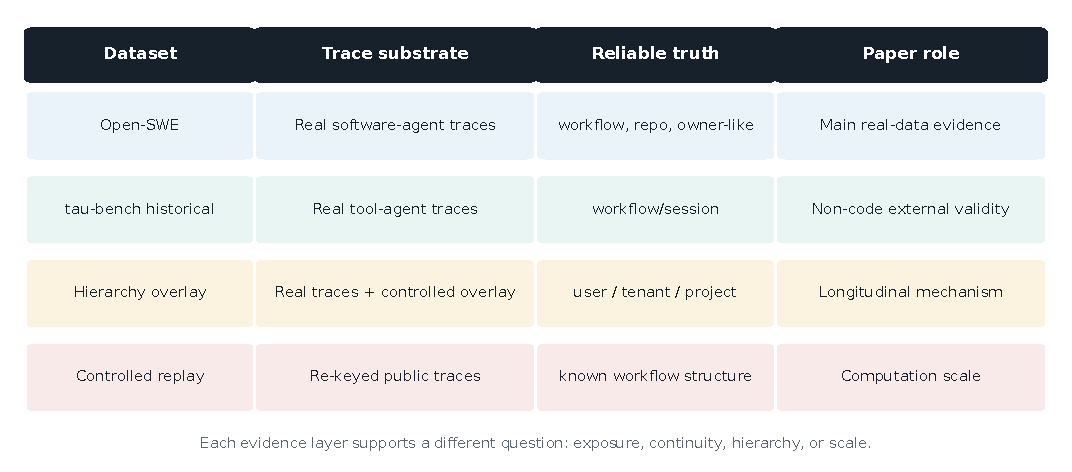
\includegraphics[width=0.98\textwidth]{figures/evidence_layers.pdf}
\caption{Evidence layers align each trace substrate and available truth with the question it can
answer: direct exposure, workflow continuity, longitudinal hierarchy, or computation scale.}
\end{figure*}

In the audited public traces, repository and owner namespace handles appear in every held-out
Open-SWE request. Historical tau-bench identity handles cover 62.6\% of requests and process handles
17.8\%; shared-resource handles cover 51.8\% but have 49.8\% cross-user ambiguity and are therefore
candidate-only. These measurements show that stable handles occur outside one code scaffold; they do
not estimate their rate in private enterprise deployments. A production study would require
consented logs, framework-stratified sampling, retention-policy metadata, and a governance process
that prevents the measurement itself from creating a new privacy risk.

\section{Learned-Representation Comparisons}

Dense MiniLM representations provide a learned comparison point. On held-out historical tau-bench,
exact dense top-$k$ linkage reaches F1 .960; HNSW with efSearch 200 reaches .956 while retaining .993
of true session pairs. On strict Open-SWE after path removal, however, dense-only project F1 is .070,
and zero-target-label cross-scaffold dense-only F1 is .037/.084. The combined sparse/dense stage is
stronger but still loses recall under scaffold shift.

Supervised pair matchers such as Ditto assume labeled match/non-match record pairs and a stable
record schema. The paper's primary attacker is cold-start, has no target registry, and must output
streaming multi-level partitions. A supervised matcher would therefore change the attacker-knowledge
assumption. We report unsupervised learned representations and ANN retrieval as in-scope baselines;
supervised entity matching is an important stronger-attacker extension rather than evidence that
CARP dominates the entity-resolution literature.

\section{Additional Robustness Interpretation}

The held-out context sweep retains candidate recall 1.000 for pair budgets 100--800. Jaccard changes
from .16 to .24 leave F1 at .910, while containment changes from .62 to .94 move F1 from .981 to
.572. The main sensitive engineering choice is therefore the required degree of context growth.
In the controlled tau overlay, complete later-alias rotation reduces user/project/tenant watchlist F1
to zero; removing all occurrences of the stable handles also gives zero. These results are empirical
counterparts to the observation-equivalence analysis: linkage fails as stable differentiating
information is removed or made exchangeable.

\end{document}
